
\chapter{Formal Concept Analysis}
\label{cha:form-conc-analys}

\todo[inline]{Write: introductory text, some historical notes, some subfield classification}

\section{Concept Lattices and Galois Connections}
\label{sec:form-cont-cont}

We introduce the basic notions of formal concept analysis in this section.  Most
importantly, we shall discuss how formal concept analysis allows us to represent
complete lattices in terms of \emph{formal concept lattices} using the notion of
\emph{formal contexts}.  Moreover, we shall introduce the notion of a \emph{Galois
  connection} between two ordered sets.

Let us briefly repeat the basic notions of order theory which are relevant for our further
considerations.  Let $P$ be a set and let ${\le} \subseteq P \times P$ be a binary
relation on $P$.  Then the pair $(P, \le)$ is called an \emph{(partially) ordered set} if
$\le$ is reflexive, transitive and antisymmetric.  Such structures can be visualize in
terms of \emph{order diagrams} (often called \emph{Hasse diagrams}) if they are finite
(and not too large).  For this way call two elements $x, y \in P$ with $x < y$
\emph{directly neighbored} in $(P, \le)$ if and only if there does not exist an element $z
\in P$ such that $x < z < y$.  Then to visualize $(P, \le)$ we mark for every element
$x \in P$ a node $v_x$ on the plane such that whenever $x < y$ it is true that the
ordinate (the second coordinate) of $v_x$ is strictly smaller then the one of $v_y$.
Then, we draw for every two elements $x, y$ with $x < y$ which are directly neighbored in
$(P, \le)$ an undirected line from $v_x$ to $v_y$.

Observe that this construction is not unique, and are many different possibilities (good
and bad) to visualize ordered sets in this way.  Also note that the naming $v_x$ of
vertices for elements $x$ is arbitrary and can be chosen as it suits.

\begin{Example}
  \label{expl:1}
  Let us consider the set $\set{1, 2, 3}$ with the usual order $\le$ on natural numbers.
  Then a line diagram of this order set is
  \begin{center}
    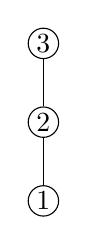
\begin{tikzpicture}[every node/.style = {draw, circle, inner sep = 1pt}]
      \node (A) {$3$};
      \node[below of=A] (B) {$2$};
      \node[below of=B] (C) {$1$};
      \draw (A) -- (B);
      \draw (B) -- (C);
    \end{tikzpicture}
  \end{center}
  We can readily read of this diagram that $1 < 2$ and $2 < 3$, because there are lines
  connecting the corresponding vertices.  But we can also see that $1 < 3$ because there
  is an \emph{ascending path} from $1$ to $3$.
\end{Example}

More generally, in a line diagram of an ordered set $(P, \le)$, two elements $x, y \in P$
satisfy $x \le y$ if and only if there is an ascending path from $x$ to $y$ in the line
diagram (where also paths of length 0 are allowed).

\begin{Example}
  \label{expl:2}
  Let $P = \set{ 1, 2, 3 }$ and consider the ordered set $(\subsets{\set{1,2,3}},
  \subseteq)$, where $\subsets{\set{1,2,3}}$ denotes the set of all subsets of
  $\set{1,2,3}$.  This set can be visualized as a line diagram as follows:
  \begin{center}
    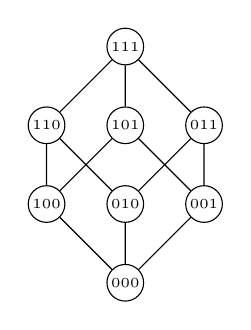
\begin{tikzpicture}[every node/.style = {draw, circle, inner sep = 1pt}]
      \node (0) at (0,0)  {\tiny 000};
      \node (1) at (-1,1) {\tiny 100};
      \node (2) at (0, 1) {\tiny 010};
      \node (3) at (1, 1) {\tiny 001};
      \node (4) at (-1,2) {\tiny 110};
      \node (5) at (0,2)  {\tiny 101};
      \node (6) at (1,2)  {\tiny 011};
      \node (7) at (0,3)  {\tiny 111};
      \draw{
        (0) -- (1)
        (0) -- (2)
        (0) -- (3)
        (1) -- (4)
        (1) -- (5)
        (2) -- (4)
        (2) -- (6)
        (3) -- (5)
        (3) -- (6)
        (4) -- (7)
        (5) -- (7)
        (6) -- (7)
      };
    \end{tikzpicture}
  \end{center}
  Here we denote subsets of $\set{1,2,3}$ by sequences of 0 and 1, meaning that if the
  first position is 1 if and only if the number 1 is an element of the corresponding
  subset, and so on.  Then 101 corresponds to the set $\set{1,3}$.
\end{Example}

An element $x \in P$ is said to be the \emph{smallest element} of $(P, \le)$ if and only
if $x \le y$ is true for all $y \in P$.  Likewise, $x$ is the \emph{greatest element} of
$(P, \le)$ if and only if $y \le x$ is true for all $y \in P$.  Note that neither smallest
nor greatest elements have to exist in $P$.  However, if these elements exist, they are
unique up to equivalence.

Let $Q \subseteq P$.  An element $x \in Q$ is said to be the \emph{smallest element} in
$Q$ (with respect to $(P, \le)$) if and only if $x \le y$ is true for all $y \in Q$;
\emph{greatest element} in $Q$ are defined likewise.  Again, neither smallest nor greatest
elements in $Q$ have to exist.

Let $x \in P$.  The \emph{order-ideal} ${\downarrow}x$ and the \emph{order-filter}
${\uparrow} x$ of $x$ in $(P, \le)$ are defined as
\begin{align*}
  {\downarrow} x &:= \set{ y \in P \mid y \le x },\\
  {\uparrow} x &:= \set{ y \in P \mid x \le y }.
\end{align*}
In other words, ${\downarrow} x$ contains all elements which are \emph{below} $x$ in $(P,
\le)$, and ${\uparrow} x$ contains all elements which are \emph{above} $x$ in $(P, \le)$.

Let again $Q \subseteq P$.  Then the sets ${\downarrow} Q$ and ${\uparrow} Q$ defined as
\begin{align*}
  {\uparrow} Q &:= \bigcap_{q \in Q} {\uparrow} q,\\
  {\downarrow} Q &:= \bigcap_{q \in Q} {\downarrow} q
\end{align*}
are called the set of \emph{upper bounds} and \emph{lower bounds} of $Q$ in $(P, \le)$,
respectively, where we employ the convention that $\bigcap \emptyset = P$.  If ${\uparrow}
Q$ has a smallest element (a \emph{least upper bound}) in $(P, \le)$, it is called the
\emph{supremum} of $Q$ in $(P, \le)$ and is denoted by $\sup Q$.  Likewise, if
${\downarrow} Q$ has a greatest element (a \emph{greatest lower bound}) in $(P, \le)$,
then it is called the \emph{infimum} of $Q$ in $(P, \le)$ and is denoted by $\inf Q$.

Note again that neither infimum nor supremum have to exist in $(P, \le)$.

\begin{Example}
  \label{expl:3}
  Let $P = \set{ a, b, c }$ and let $\le$ be given by the smallest order relation that
  satisfies $a < b$ and $a < c$.  Then $\inf\set{b,c}$ exists in $(P, \le)$ and is equal
  to $a$.  However, $\sup\set{b, c}$ does not exist in $(P, \le)$, as ${\uparrow} b \cap
  {\uparrow} c = \emptyset$.
\end{Example}

\noindent%
Structures in which supremum and infimum always exist for \emph{finite} sets $Q$ are
called \emph{lattices}.  If the sets $Q$ can be chosen arbitrary, then we call such a
structure a \emph{complete lattice}.

\begin{Definition}[Lattice]
  \label{def:lattice}
  Let $\mathbb L = (L, \le)$ be an ordered set.  Then $\mathbb L$ is called a
  \emph{lattice} if and only if for each finite $Q \subseteq L$ there exist both $\sup Q$
  and $\inf Q$ in $\mathbb L$.  If for all $Q \subseteq L$ there exist both $\sup Q$ and
  $\inf Q$ in $\mathbb L$, then $\mathbb L$ is called a \emph{complete lattice}.
\end{Definition}

\noindent%
Note that every finite lattice is also a complete lattice.  Moreover, every complete
lattice has a smallest and greatest element, given by $\sup\emptyset$ and $\inf\emptyset$,
respectively.  Furthermore, every ordered set $(P, \le)$ in which the supremum exists for
each $Q \subseteq P$ is already a complete lattice, as the infimum is then given by
\begin{equation*}
  \inf Q = \sup\set{ x \in P \mid \forall y \in Q \holds x \le y }.
\end{equation*}
The same is of course true if supremum and infimum are exchanged.

The ordered sets from Examples~\ref{expl:1} and~\ref{expl:2} are lattices, but not the one
from~\ref{expl:3}.  More generally, if $P$ is a set, then $(\subsets{P}, \subseteq)$ is
always a complete lattice.

The study of lattices as mathematical structures has received much interest over the last
decades and thus constitutes a major branch of order theory.\todo{cite main book on
  lattice theory} However, (complete) lattices also allow for a quite natural
interpretation as a hierarchy of \emph{generalizations} and \emph{specializations}: an
element $x$ is below an element $y$ if and only if $x$ is more \emph{special} than $y$, or
alternatively, if $y$ is more \emph{general} than $x$.  Then for a set $Q$ of elements its
supremum $\sup Q$ can be thought of as a \emph{most-specific generalization} of all
elements in $Q$, and $\inf Q$ can be seen likewise as the most \emph{general
  specialization} of all elements in $Q$.

Formal concept analysis now provides an approach to understand complete lattice in terms
of this interpretation, by representing these lattices in terms of \emph{objects} and
their \emph{attributes}.  For this, we need to introduce the notion of a \emph{formal
  context}.

\begin{Definition}[Formal Context]
  \label{def:formal-context}
  A \emph{formal context} $\con K$ is constituted of three sets $G, M, I$, where $I
  \subseteq G \times M$.  Most often, we shall identify $\con K$ with the triple $(G, M,
  I)$, \ie $\con K = (G, M, I)$.  We shall call $G$ the set of \emph{objects} of $\con K$,
  $M$ the set of \emph{attributes} of $\con K$ and $I$ the \emph{incidence} of $\con K$.
  Two formal contexts are equal if and only if their sets of objects, attributes and their
  incidences are equal, respectively.
\end{Definition}

Formal contexts can be thought of as simple data structures which record for a set of
objects the set of attributes those objects have.  More precisely, we shall say that in a
formal context $\con K$ an object $g \in G$ \emph{has} an attribute $m$ if and only if
$(g, m) \in I$.

\begin{Example}
  \label{sec:conc-latt-galo}
  Let us consider a small toy example $\con K_{\mathsf{TNG}}$ to illustrate the definition
  of a formal context.  As sets of objects we choose some fictional characters from
  \emph{Star Trek: The Next Generation}, namely
  \begin{equation*}
    G := \set{ \mathsf{Picard}, \mathsf{Worf}, \mathsf{Data}, \mathsf{Borg Queen} }.
  \end{equation*}
  As sets of attributes we choose
  \begin{equation*}
    M := \set{ \mathsf{Human}, \mathsf{Honorable}, \mathsf{Artificial}, \mathsf{Star
        Fleet} }.
  \end{equation*}
  To illustrate the incidence relation of our examples formal context we make use of a
  \emph{cross table}, \ie we depict $\con K_{\mathsf{TNG}}$ as a table where the rows are
  labeled with objects and the columns are labeled with attributes.  Then in every cell we
  write a cross if and only if the objects labeling the corresponding row has the
  attribute labeling the corresponding column.
  \begin{equation*}
    \def\x{\times}
    \begin{array}{r|*{4}{c}}
      \toprule
      \con K_{\mathsf{TNG}} & \mathsf{Human} & \mathsf{Honorable} & \mathsf{Artificial} & \mathsf{Star Fleet} \\
      \midrule
      \mathsf{Picard} & \x & \x & & \x \\
      \mathsf{Worf} & & \x & & \x \\
      \mathsf{Data} & & \x & \x & \x \\
      \mathsf{Borg Queen} & & & \x & \\
      \bottomrule
    \end{array}
  \end{equation*}
  Then \textsf{Borg Queen} has the attribute \textsf{Artificial}, but not \textsf{Honorable}.
\end{Example}

To now expose the connection between formal contexts on the one hand and complete lattices
on the other we shall introduce the \emph{derivation operators} in formal contexts.

\begin{Definition}[Contextual Derivation]
  Let $\con K = (G, M, I)$ be a formal context and let $A \subseteq G$ be a set of
  objects.  Then the set of \emph{common attributes} $A'$ of $A$ is defined to be
  \begin{equation*}
    A' := \set{ m \in M \mid \forall g \in G \holds (g, m) \in I }.
  \end{equation*}
  Likewise, for a set $B \subseteq M$ of attributes we define the set $B'$ of \emph{shared
    objects} as
  \begin{equation*}
    B' := \set{ g \in G \mid \forall m \in M \holds (g, m) \in I }.
  \end{equation*}
  The functions $A \mapsto A'$ and $B \mapsto B'$ are called the \emph{derivation
    operators} of $\con K$, and the sets $A'$ and $B'$ are called the \emph{derivations}
  of $A$ and $B$ in $\con K$, respectively.
\end{Definition}

\noindent For $(A')'$ we may also simply write $A''$.

Note that both derivation operators are denoted by $(\cdot)'$, which usually does not lead
to confusion, as it is most often clear from the context whether we deal with a set of
objects or a set of attributes from which we want to compute its derivation.  If it
nevertheless happens that a single name for the derivation operator leads to confusion,
then we shall locally introduce separate names for both of them.

What occurs more often, for example in Chapters~\ref{cha:expl-conf}
and~\ref{cha:model-expl-conf}, is the derivation of sets in \emph{different contexts}.
For example we may have given two formal contexts $\con K_1 = (G_1, M_1, I_1)$ and $\con
K_2 = (G_2, M_2, I_2)$ and a set $A \subseteq M_1 \cap M_2$.  Then when writing $A'$ it is
not clear in which context we do the derivation.  To remedy this, we shall add a subscript
to the set $A$ to make clear of which context we consider it as a set of attributes:
$A_{\con K_1}$ denotes the set $A$ considered as a set of attributes in $\con K_1$, and
likewise $A_{\con K_2}$.  While this notation is not useful as it stands, it becomes handy
if we consider derivations of $A$: $(A_{\con K_1})'$ denotes the derivation of $A$ in the
formal context $\con K_1$, while $(A_{\con K_2})'$ does the same for the formal context
$\con K_2$.  Of course, we can drop the parentheses if they do not lead to ambiguity and
write $A_{\con K_1}'$ and $A_{\con K_2}'$ instead.  Of course, the same can be done for
sets of objects.  In particular, instead of writing $(A_{\con K_1}')_{\con K_1}'$ we shall
often only write $A_{\con K_1}''$.

\begin{Example}
  \label{expl:4}
  Consider our Star Trek example context from~\ref{expl:3} and let $A :=
  \set{\mathsf{Human}}$.  Then $A' = \set{ \mathsf{Picard} }$, $A'' = \set{
    \mathsf{Human}, \mathsf{Honorable}, \mathsf{Star Fleet} }$, and $A''' = \set{
    \mathsf{Picard} } = A'$.
\end{Example}

\todo[inline]{Write: Galois connections}%
\todo[inline]{Write: concept lattices}%

\section{Implications and Bases}
\label{sec:implications-sets}

\todo[inline]{Write: implications on sets}%
\todo[inline]{Write: valid implications of formal contexts}%
\todo[inline]{Write: closure operators induced by sets of implications}%
\todo[inline]{Write: bases of implications, special case of set of implications is the
  theory of a formal context}%
\todo[inline]{Write: introduce canonical base with arbitrary background knowledge}%
\todo[inline]{Write: computing the canonical base}

\section{Attribute Exploration}
\label{sec:attr-expl}

\todo[inline]{Write: introduce classical attribute exploration}%
\todo[inline]{Write: mention case of invalid background knowledge}%

%%% Local Variables: 
%%% mode: latex
%%% TeX-master: "../main"
%%% End: 

%  LocalWords:  sep
